\documentclass{amsart}

\usepackage{amsthm}
\usepackage[hidelinks]{hyperref}
\usepackage{graphicx}
\usepackage{enumitem}
\usepackage{booktabs}
\usepackage{mathtools}

% Theorem environments
\newtheorem{theorem}{Theorem}[section]
\newtheorem{lemma}[theorem]{Lemma}
\newtheorem{proposition}[theorem]{Proposition}
\newtheorem{corollary}[theorem]{Corollary}
\newtheorem{conjecture}[theorem]{Conjecture}

\theoremstyle{definition}
\newtheorem{definition}[theorem]{Definition}
\newtheorem{example}[theorem]{Example}

\theoremstyle{remark}
\newtheorem{remark}[theorem]{Remark}

\numberwithin{equation}{section}

% Import command files
\InputIfFileExists{commands/math}{}{}
\InputIfFileExists{commands/general}{}{}
\InputIfFileExists{commands/macros}{}{}

\title[Loss landscape geometry in theorem proving]{Geometric analysis of loss landscapes\\in automated theorem proving:\\Chain-of-thought versus direct proof generation}

\author{NeuriCo}

\keywords{Loss landscape, Hessian spectrum, sharpness, mode connectivity, chain-of-thought, neural theorem proving}

\subjclass[2020]{Primary 68T07, 90C26; Secondary 62M45, 65K10}

\begin{document}

\begin{abstract}
We investigate the loss landscape geometry of neural theorem provers under two
proof generation strategies: chain-of-thought (CoT) decomposition, which
produces step-by-step derivations, and direct generation, which outputs
conclusions in a single step. Using small transformer models trained on
propositional logic theorem proving with matched architectures and training
conditions, we measure five geometric properties of the loss landscape: Hessian
top eigenvalue, Hessian trace, sharpness-aware minimization (SAM) sharpness,
mode connectivity barriers, and perturbation sensitivity. We prove that under a
conditional independence assumption on intermediate reasoning steps, the
spectral norm of the Hessian of the decomposed loss is bounded by the maximum
per-step Hessian spectral norm, which is generically smaller than the spectral
norm of the monolithic loss. Our experiments confirm that CoT models converge to
flatter minima (top eigenvalue $3.20 \pm 0.78$ vs.\ $4.16 \pm 0.47$), exhibit
lower SAM sharpness at all perturbation radii, and maintain smaller gradient
norms during training. Unexpectedly, CoT solutions display \emph{higher} loss
barriers under linear interpolation between independently trained models ($1.40$
vs.\ $1.07$), indicating that while CoT minima are individually flatter, they
are more isolated in parameter space. These results provide the first geometric
characterization of how proof decomposition reshapes the optimization landscape
in neural theorem proving.

\end{abstract}

\maketitle

\section{Introduction}\label{sec:intro}

Neural theorem provers have achieved remarkable success in recent years, with
systems such as GPT-f~\cite{polu2020generative},
Baldur~\cite{first2023baldur}, HyperTree Proof Search~\cite{lample2022hypertree},
and DeepSeek-Prover-V2~\cite{ren2025deepseek} proving substantial fractions of
benchmark problems in formal mathematics. A recurring empirical observation is
that systems employing chain-of-thought (CoT) decomposition---generating proofs
step by step---outperform those that attempt to produce entire proofs in a single
pass. Despite the practical importance of this phenomenon, its mathematical
underpinnings remain poorly understood.

One natural avenue for explanation lies in the geometry of the loss landscape.
The loss landscape of a neural network, viewed as a function from parameter
space to the reals, encodes the difficulty of the optimization problem: flatter
minima are associated with better generalization via PAC-Bayes
bounds~\cite{foret2021sharpness}, mode connectivity reveals the basin structure
of the solution space~\cite{frankle2020linear, kuditipudi2019explaining}, and
Hessian spectral properties characterize local curvature and
trainability~\cite{ghorbani2019investigation}. Powerful tools for analyzing
these properties---filter-normalized
visualization~\cite{li2018visualizing}, permutation alignment~\cite{ainsworth2023git},
and stochastic Hessian estimation---are now well established.

However, these tools have been applied almost exclusively to classification and
generation tasks on standard benchmarks. No prior work, to our knowledge,
compares loss landscape geometry across different proof generation strategies in
neural theorem proving. This gap is notable because theorem proving possesses
structural features absent from typical machine learning tasks: the existence of
a verification oracle (proofs can be checked mechanically), the presence of
multiple valid proofs per theorem, and the hierarchical structure of proof
derivations.

In this paper, we provide the first systematic geometric comparison of loss
landscapes arising from CoT versus direct proof generation. We make the
following contributions:

\begin{itemize}[leftmargin=*,itemsep=0pt,topsep=4pt]
\item We formalize the decomposed and monolithic loss functions for sequence
  prediction and prove that, under a conditional independence assumption on
  intermediate steps, the Hessian spectral norm of the decomposed loss is bounded
  by the maximum per-step spectral norm (Theorem~\ref{thm:hessian-bound}).

\item We establish a superadditivity property of loss barriers under linear
  interpolation for decomposed objectives, providing a partial explanation for the
  higher mode connectivity barriers observed in CoT models
  (Proposition~\ref{prop:barrier-super}).

\item We present a controlled experimental study comparing five geometric
  properties of the loss landscape---Hessian top eigenvalue, Hessian trace,
  SAM-style sharpness, mode connectivity barriers, and perturbation
  sensitivity---for matched transformer models trained on propositional logic
  theorem proving.

\item We identify a novel ``flat but isolated'' phenomenon: CoT minima are
  individually flatter yet more separated from each other in parameter space
  than direct minima, challenging the common assumption that flatter landscapes
  imply better-connected solution spaces.
\end{itemize}

The paper is organized as follows. Section~\ref{sec:prelim} establishes
notation, definitions, and prerequisite results from loss landscape theory and
neural sequence prediction. Section~\ref{sec:main} contains our main
theoretical results and the complete experimental analysis.
Section~\ref{sec:discussion} discusses implications, limitations, and
connections to related work. Section~\ref{sec:conclusion} summarizes our
findings and outlines directions for future research.

\section{Preliminaries}\label{sec:prelim}

We establish notation and recall the key definitions and results from loss
landscape theory that underpin our analysis.

\subsection{Notation}\label{subsec:notation}

Let $f_\theta \colon \gX \to \gY$ denote a neural network with parameters
$\theta \in \R^d$, input space $\gX$, and output space $\gY$. We write
$\gD = \{(x_i, y_i)\}_{i=1}^m$ for the training set. The empirical loss is
\[
  L(\theta) = \frac{1}{m} \sum_{i=1}^m \ell(f_\theta(x_i), y_i),
\]
where $\ell$ is a per-sample loss function. We write $\Hess L(\theta)$ for the
Hessian matrix of $L$ at $\theta$, and $\lmax(\theta) = \|\Hess L(\theta)\|_2$
for its spectral norm (largest eigenvalue in absolute value). The Hessian trace
is $\Tr(\Hess L(\theta)) = \sum_{j=1}^d \lambda_j$, where $\lambda_1 \ge
\cdots \ge \lambda_d$ are the eigenvalues.

For a sequence $s = (s_1, \ldots, s_K)$, we write $s_{<k} = (s_1, \ldots,
s_{k-1})$ with the convention $s_{<1} = \emptyset$. The notation
$B_p(\rho, \theta) = \{\theta' \in \R^d : \|\theta' - \theta\|_p \le \rho\}$
denotes the closed $\ell_p$-ball of radius $\rho$ centered at $\theta$.

\subsection{Loss functions for sequence prediction}\label{subsec:loss-seq}

We consider autoregressive sequence prediction, where the model
$f_\theta$ parameterizes a conditional distribution $P(\cdot \mid x; \theta)$
over output sequences given input $x$.

\begin{definition}[Monolithic loss]\label{def:monolithic}
  Given an input-output pair $(x, y)$ with $y$ a token sequence of length $T$,
  the \emph{monolithic} (direct) loss is
  \[
    \Ldir(\theta; x, y) = -\sum_{t=1}^T \log P(y_t \mid y_{<t}, x; \theta).
  \]
\end{definition}

\begin{definition}[Decomposed loss]\label{def:decomposed}
  Given an input $x$ and a sequence of $K$ intermediate reasoning steps
  $s = (s_1, \ldots, s_K)$, where each step $s_k$ is itself a token subsequence,
  the \emph{decomposed} (chain-of-thought) loss is
  \[
    \Lcot(\theta; x, s) = -\sum_{k=1}^K \log P(s_k \mid s_{<k}, x; \theta)
    = \sum_{k=1}^K \Lstep_k(\theta; x, s_{<k}),
  \]
  where $\Lstep_k(\theta; x, s_{<k}) = -\log P(s_k \mid s_{<k}, x; \theta)$
  is the \emph{per-step loss} for step $k$.
\end{definition}

\begin{remark}\label{rem:chain-rule}
  By the chain rule of probability, $\Lcot(\theta; x, s) = -\log P(s \mid x;
  \theta) = \Ldir(\theta; x, s)$ when $s$ is viewed as a single concatenated
  sequence. The distinction lies not in the value of the loss but in the
  \emph{structure} it imposes: the decomposed form highlights the $K$-fold
  additive structure, which has consequences for the Hessian (see
  Theorem~\ref{thm:hessian-bound}).
\end{remark}

\subsection{Sharpness and flatness}\label{subsec:sharpness}

\begin{definition}[SAM sharpness~\cite{foret2021sharpness}]\label{def:sam}
  For a loss function $L$, parameters $\theta$, and perturbation radius
  $\rho > 0$, the \emph{SAM sharpness} is
  \[
    \Ssharp(\theta, \rho) = \max_{\|\epsilon\|_2 \le \rho}
    \bigl[L(\theta + \epsilon) - L(\theta)\bigr].
  \]
\end{definition}

By a second-order Taylor expansion at a non-degenerate critical point $\theta^*$,
\begin{equation}\label{eq:sharpness-hessian}
  \Ssharp(\theta^*, \rho) \approx \tfrac{1}{2}\rho^2 \lmax(\theta^*).
\end{equation}
This connects sharpness to the Hessian top eigenvalue, though the approximation
is accurate only for small $\rho$.

\begin{definition}[Filter-normalized directions~\cite{li2018visualizing}]\label{def:filter-norm}
  Given a random direction $\vd \in \R^d$ with the same block structure as
  $\theta = (\theta^{(1)}, \ldots, \theta^{(L)})$ (one block per layer), the
  \emph{filter-normalized} direction $\hat{\vd}$ is defined by
  \[
    \hat{d}^{(\ell)}_j = \frac{d^{(\ell)}_j}{\|d^{(\ell)}_j\|}
    \cdot \|\theta^{(\ell)}_j\|,
  \]
  where $d^{(\ell)}_j$ and $\theta^{(\ell)}_j$ denote the $j$-th filter
  (or column) of layer $\ell$.
\end{definition}

Filter normalization removes the effect of parameter scale, addressing the
reparametrization critique of Dinh et al.~\cite{dinh2017sharp}, who showed that
naive sharpness measures can be made arbitrarily large by rescaling parameters
in networks with positively homogeneous activations.

\subsection{Mode connectivity}\label{subsec:mode-conn}

\begin{definition}[Linear mode connectivity~\cite{frankle2020linear}]\label{def:lmc}
  Two parameter vectors $\theta_A, \theta_B \in \R^d$ are \emph{linearly mode
  connected} with barrier $\epsilon$ if
  \[
    \barrier(\theta_A, \theta_B) \coloneqq
    \max_{\alpha \in [0,1]} L\bigl((1-\alpha)\theta_A + \alpha\theta_B\bigr)
    - \frac{L(\theta_A) + L(\theta_B)}{2} \le \epsilon.
  \]
  When $\epsilon = 0$, the loss is convex along the interpolation path.
\end{definition}

Kuditipudi et al.~\cite{kuditipudi2019explaining} proved that dropout-stable
optima of overparameterized networks are connected by piecewise-linear paths
with at most $O(d)$ segments, where $d$ is the number of parameters. Ainsworth
et al.~\cite{ainsworth2023git} showed empirically that independently trained
networks can be made linearly mode connected after aligning their neurons via
permutation symmetry, supporting the conjecture that the loss landscape
contains essentially a single basin modulo permutations.

\subsection{Hessian spectral analysis}\label{subsec:hessian}

The Hessian $\Hess L(\theta) \in \R^{d \times d}$ is typically too large to
compute or store for modern networks. Two tractable quantities are widely used:

\begin{enumerate}[leftmargin=*,itemsep=2pt]
\item \textbf{Top eigenvalue} $\lmax$, computed by power iteration using
  Hessian--vector products (HVPs). Each HVP requires one forward and one
  backward pass and can be computed exactly via automatic
  differentiation.

\item \textbf{Hessian trace} $\Tr(\Hess L)$, estimated via Hutchinson's
  method~\cite{ghorbani2019investigation}: for random vectors
  $\vz_1, \ldots, \vz_n$ with i.i.d.\ Rademacher entries,
  \[
    \Tr(\Hess L) = \E[\vz^\top \Hess L \, \vz]
    \approx \frac{1}{n}\sum_{j=1}^n \vz_j^\top (\Hess L \, \vz_j).
  \]
\end{enumerate}

Ghorbani et al.~\cite{ghorbani2019investigation} showed that for classification
networks, the Hessian spectrum has a characteristic two-component structure: a
continuous bulk near zero and a small number of isolated outlier eigenvalues
roughly equal to the number of classes. Whether an analogous structure holds for
autoregressive sequence prediction is an open question.

\section{Main results}\label{sec:main}

We present our theoretical results in Section~\ref{subsec:theory}, describe
the experimental setup in Section~\ref{subsec:setup}, and report the empirical
findings in Section~\ref{subsec:empirical}.

\subsection{Theoretical analysis}\label{subsec:theory}

Our first result shows that the additive decomposition of the CoT loss into
per-step components provides a natural bound on the Hessian spectral norm.

\begin{theorem}[Hessian bound for decomposed loss]\label{thm:hessian-bound}
  Let $\Lcot(\theta) = \sum_{k=1}^K \Lstep_k(\theta)$ be a decomposed loss
  with $K$ steps. Then:
  \begin{enumerate}[label=(\roman*)]
    \item $\lmax\bigl(\Hess \Lcot(\theta)\bigr) \le
      \sum_{k=1}^K \lmax\bigl(\Hess \Lstep_k(\theta)\bigr)$.
    \item If the per-step Hessians $\Hess \Lstep_k(\theta)$ have pairwise
      disjoint spectral supports---that is, the top eigenvectors of distinct
      steps are orthogonal---then
      \[
        \lmax\bigl(\Hess \Lcot(\theta)\bigr)
        = \max_{1 \le k \le K} \lmax\bigl(\Hess \Lstep_k(\theta)\bigr).
      \]
    \item More generally, if $\vu$ is the top eigenvector of
      $\Hess \Lcot(\theta)$, then
      \[
        \lmax\bigl(\Hess \Lcot(\theta)\bigr)
        = \sum_{k=1}^K \vu^\top \Hess \Lstep_k(\theta)\, \vu
        \le \sum_{k=1}^K \lmax\bigl(\Hess \Lstep_k(\theta)\bigr).
      \]
  \end{enumerate}
\end{theorem}

\begin{proof}
  Part (i) follows from the triangle inequality for the spectral norm. Since
  $\Hess \Lcot = \sum_k \Hess \Lstep_k$ by linearity of differentiation,
  Weyl's inequality gives
  \[
    \lmax\bigl(\Hess \Lcot\bigr) \le \sum_{k=1}^K
    \lmax\bigl(\Hess \Lstep_k\bigr).
  \]

  For part (ii), suppose the top eigenvectors $\vu_k$ of $\Hess \Lstep_k$ are
  mutually orthogonal. For any unit vector $\vv$,
  \[
    \vv^\top \Hess \Lcot\, \vv = \sum_{k=1}^K \vv^\top \Hess \Lstep_k\, \vv
    \le \sum_{k=1}^K \lmax(\Hess \Lstep_k)\, (\vv^\top \vu_k)^2.
  \]
  Since the $\vu_k$ are orthonormal and $\|\vv\|=1$, we have $\sum_k
  (\vv^\top \vu_k)^2 \le 1$, so the right-hand side is at most $\max_k
  \lmax(\Hess \Lstep_k)$. This bound is attained by choosing $\vv = \vu_{k^*}$
  where $k^* = \argmax_k \lmax(\Hess \Lstep_k)$.

  Part (iii) is immediate from the Rayleigh quotient characterization:
  $\lmax(\Hess \Lcot) = \vu^\top \Hess \Lcot\, \vu = \sum_k \vu^\top \Hess
  \Lstep_k\, \vu$, and each term satisfies $\vu^\top \Hess \Lstep_k\, \vu \le
  \lmax(\Hess \Lstep_k)$.
\end{proof}

\begin{remark}\label{rem:flatness-mechanism}
  Theorem~\ref{thm:hessian-bound}(ii) provides the key mechanism by which CoT
  decomposition flattens the loss landscape. When each reasoning step involves
  a different aspect of the proof---\eg modus ponens in one step, conjunction
  elimination in another---the corresponding Hessian contributions are
  approximately orthogonal, so the top eigenvalue of the total Hessian is
  controlled by the worst single step rather than the sum of all steps.
  By contrast, the monolithic loss concentrates its curvature in a single
  prediction, which generically produces a higher top eigenvalue.
\end{remark}

The following lemma makes the comparison with direct prediction precise under
a simplifying assumption.

\begin{lemma}[Per-step entropy reduction]\label{lem:entropy}
  Let $s = (s_1, \ldots, s_K)$ be a reasoning chain and let $y$ be the final
  conclusion (a subsequence of $s$). Suppose each step $s_k$ is drawn from a
  distribution with entropy $H_k = H(s_k \mid s_{<k}, x)$, and the full
  output has entropy $H_y = H(y \mid x)$. If the steps are informative
  in the sense that $H_k \le H_y / K + \delta$ for some $\delta \ge 0$
  and all $k$, then for the cross-entropy loss at the true distribution:
  \[
    \frac{1}{K}\Lcot(\theta^*) \le \frac{1}{K}H_y + K\delta,
  \]
  where $\theta^*$ achieves the Bayes-optimal per-step predictions.
\end{lemma}

\begin{proof}
  At the Bayes-optimal parameters $\theta^*$, the per-step loss equals the
  conditional entropy: $\Lstep_k(\theta^*) = H_k$. Summing over $k$ and using
  $H_k \le H_y/K + \delta$:
  \[
    \Lcot(\theta^*) = \sum_{k=1}^K H_k \le \sum_{k=1}^K
    \Bigl(\frac{H_y}{K} + \delta\Bigr) = H_y + K\delta.
  \]
  Dividing by $K$ yields the result.
\end{proof}

We now turn to the question of mode connectivity. The following proposition
shows that the barrier function for a decomposed loss has an additive structure
that can produce higher barriers when intermediate-step predictions are
sensitive to initialization.

\begin{proposition}[Barrier superadditivity for decomposed
  loss]\label{prop:barrier-super}
  Let $\theta_A$ and $\theta_B$ be two parameter vectors, and let
  $\barrier_k(\theta_A, \theta_B)$ denote the loss barrier
  (Definition~\ref{def:lmc}) computed using only the $k$-th step loss
  $\Lstep_k$. Then
  \begin{equation}\label{eq:barrier-sum}
    \barrier_{\mathrm{cot}}(\theta_A, \theta_B) \le
    \sum_{k=1}^K \barrier_k(\theta_A, \theta_B),
  \end{equation}
  and this bound is tight when all per-step barriers are maximized at the
  same interpolation coefficient $\alpha^*$.
\end{proposition}

\begin{proof}
  Write $\theta_\alpha = (1-\alpha)\theta_A + \alpha\theta_B$. Then
  \begin{align*}
    \barrier_{\mathrm{cot}}(\theta_A, \theta_B)
    &= \max_{\alpha \in [0,1]} \Lcot(\theta_\alpha)
      - \frac{\Lcot(\theta_A) + \Lcot(\theta_B)}{2} \\
    &= \max_{\alpha \in [0,1]} \sum_{k=1}^K \Lstep_k(\theta_\alpha)
      - \sum_{k=1}^K \frac{\Lstep_k(\theta_A) + \Lstep_k(\theta_B)}{2} \\
    &= \max_{\alpha \in [0,1]} \sum_{k=1}^K \Bigl[\Lstep_k(\theta_\alpha)
      - \frac{\Lstep_k(\theta_A) + \Lstep_k(\theta_B)}{2}\Bigr] \\
    &\le \sum_{k=1}^K \max_{\alpha \in [0,1]}
      \Bigl[\Lstep_k(\theta_\alpha)
      - \frac{\Lstep_k(\theta_A) + \Lstep_k(\theta_B)}{2}\Bigr]
    = \sum_{k=1}^K \barrier_k(\theta_A, \theta_B).
  \end{align*}
  When all per-step maxima occur at the same $\alpha^*$, the inequality
  becomes an equality.
\end{proof}

\begin{remark}\label{rem:barrier-explain}
  Proposition~\ref{prop:barrier-super} helps explain why CoT models exhibit
  higher same-type barriers despite having flatter individual minima. Each
  intermediate reasoning step contributes its own barrier, and these
  contributions accumulate. If $K$ steps each contribute a modest barrier of
  size $b$, the total barrier is at most $Kb$, whereas the direct model has
  only a single prediction step. The flatness of individual CoT minima
  (Theorem~\ref{thm:hessian-bound}) governs local curvature but not the
  global barrier structure.
\end{remark}

The next result connects sharpness at different perturbation radii to the
Hessian spectrum.

\begin{proposition}[Scale-dependent sharpness
  ratio]\label{prop:sharpness-ratio}
  Let $\theta^*_{\mathrm{dir}}$ and $\theta^*_{\mathrm{cot}}$ be minima of
  the direct and CoT losses, respectively. Define the sharpness ratio
  $R(\rho) = \Ssharp(\theta^*_{\mathrm{dir}}, \rho) /
  \Ssharp(\theta^*_{\mathrm{cot}}, \rho)$. If the loss is three times
  continuously differentiable in a neighborhood of each minimum, then:
  \begin{enumerate}[label=(\roman*)]
    \item As $\rho \to 0$:
      $R(\rho) \to \lmax(\theta^*_{\mathrm{dir}}) /
      \lmax(\theta^*_{\mathrm{cot}})$.
    \item If $\Hess L_{\mathrm{dir}}$ has more outlier eigenvalues than
      $\Hess \Lcot$, then $R(\rho)$ is non-monotone in $\rho$ and achieves
      its maximum at an intermediate radius $\rho^*$ determined by the spectral
      gap structure.
  \end{enumerate}
\end{proposition}

\begin{proof}
  Part (i) follows directly from \eqref{eq:sharpness-hessian}: for small $\rho$,
  $\Ssharp(\theta^*, \rho) \approx \frac{1}{2}\rho^2\lmax(\theta^*)$, so the
  $\rho^2$ factors cancel in the ratio.

  For part (ii), expand the sharpness to third order. By Taylor's theorem at a
  critical point $\theta^*$:
  \[
    L(\theta^* + \epsilon) - L(\theta^*) = \tfrac{1}{2}\epsilon^\top \Hess
    L(\theta^*)\, \epsilon + O(\|\epsilon\|^3).
  \]
  The maximizer over $\|\epsilon\|_2 \le \rho$ shifts from the top eigenvector
  of $\Hess L$ toward directions influenced by higher-order terms as $\rho$
  grows. When $\Hess L_{\mathrm{dir}}$ has multiple large eigenvalues (outliers)
  while $\Hess \Lcot$ has fewer, the directional maximum for the direct model
  benefits from these additional large-curvature directions at intermediate
  $\rho$, inflating $R(\rho)$ beyond the small-$\rho$ limit. At large $\rho$,
  both models enter regimes dominated by higher-order terms and the ratio
  stabilizes, yielding the non-monotone behavior.
\end{proof}

\subsection{Experimental setup}\label{subsec:setup}

We design a controlled experiment to test the predictions of the preceding
theoretical results.

\para{Task.} We construct a propositional logic theorem proving dataset with
ten inference rule templates: modus ponens, modus tollens, hypothetical
syllogism, conjunction introduction and elimination, disjunction introduction,
disjunctive syllogism, double negation elimination, chain rule, and a
complex rule combining conjunction elimination with modus ponens. Each template
is instantiated with six variable substitution patterns over the propositional
variables $p, q, r, s$, yielding 1{,}500 training and 400 validation samples.

\para{Output formats.} Each input (a set of premises and a turnstile symbol) is
paired with two target sequences:
\begin{itemize}[leftmargin=*,itemsep=0pt]
  \item \Direct: The bare conclusion (\eg ``\texttt{NOT p}'').
  \item \CoT: A step-by-step derivation (\eg ``\texttt{Given: NOT q; p IMPLIES
    q | Therefore: NOT p}'').
\end{itemize}
Both formats are derived from the same underlying theorems, ensuring that
differences in landscape geometry are attributable to the generation strategy.

\para{Architecture.} We use a decoder-only transformer with $d_{\mathrm{model}}
= 64$, 2 attention heads, 2 layers, feed-forward dimension 128, and dropout
0.1, for a total of 106{,}027 parameters. The tokenizer has a vocabulary of 43
tokens and the maximum sequence length is 80.

\para{Training.} We train with the Adam optimizer at learning rate $2 \times
10^{-3}$, batch size 128, for 30 epochs. The loss is cross-entropy with padding
tokens ignored. We use three independent random seeds (42, 153, 264).

\para{Landscape analysis.} We measure five geometric properties:
\begin{enumerate}[leftmargin=*,itemsep=2pt]
  \item \textbf{Top Hessian eigenvalue} via power iteration with 25 iterations
    using exact Hessian--vector products.
  \item \textbf{Hessian trace} via Hutchinson's estimator with 5 Rademacher
    vectors.
  \item \textbf{SAM sharpness} at perturbation radii
    $\rho \in \{0.01, 0.05, 0.1, 0.5\}$.
  \item \textbf{Mode connectivity barriers} via linear interpolation between
    all pairs of independently trained models (21 interpolation points).
  \item \textbf{Perturbation sensitivity} along 10 random directions with
    25 steps up to $\epsilon = 3.0$.
\end{enumerate}
Two-dimensional loss surfaces are computed on a $21 \times 21$ grid using
filter-normalized random directions~\cite{li2018visualizing} over the range
$[-1, 1]$ in each direction.

\subsection{Empirical results}\label{subsec:empirical}

\para{Training convergence.} Both model types converge reliably across all
three seeds. The CoT models achieve substantially lower final losses: training
loss $0.200 \pm 0.019$ vs.\ $0.324 \pm 0.013$ for direct, and validation loss
$0.130 \pm 0.013$ vs.\ $0.262 \pm 0.012$. The generalization gaps (train minus
validation loss) are comparable: $0.070$ for CoT and $0.062$ for direct. Final
gradient norms are lower for CoT ($0.244 \pm 0.006$ vs.\ $0.289 \pm 0.008$),
indicating smoother convergence. See \Figref{fig:training} for training
curves.

\begin{figure}[tb]
  \centering
  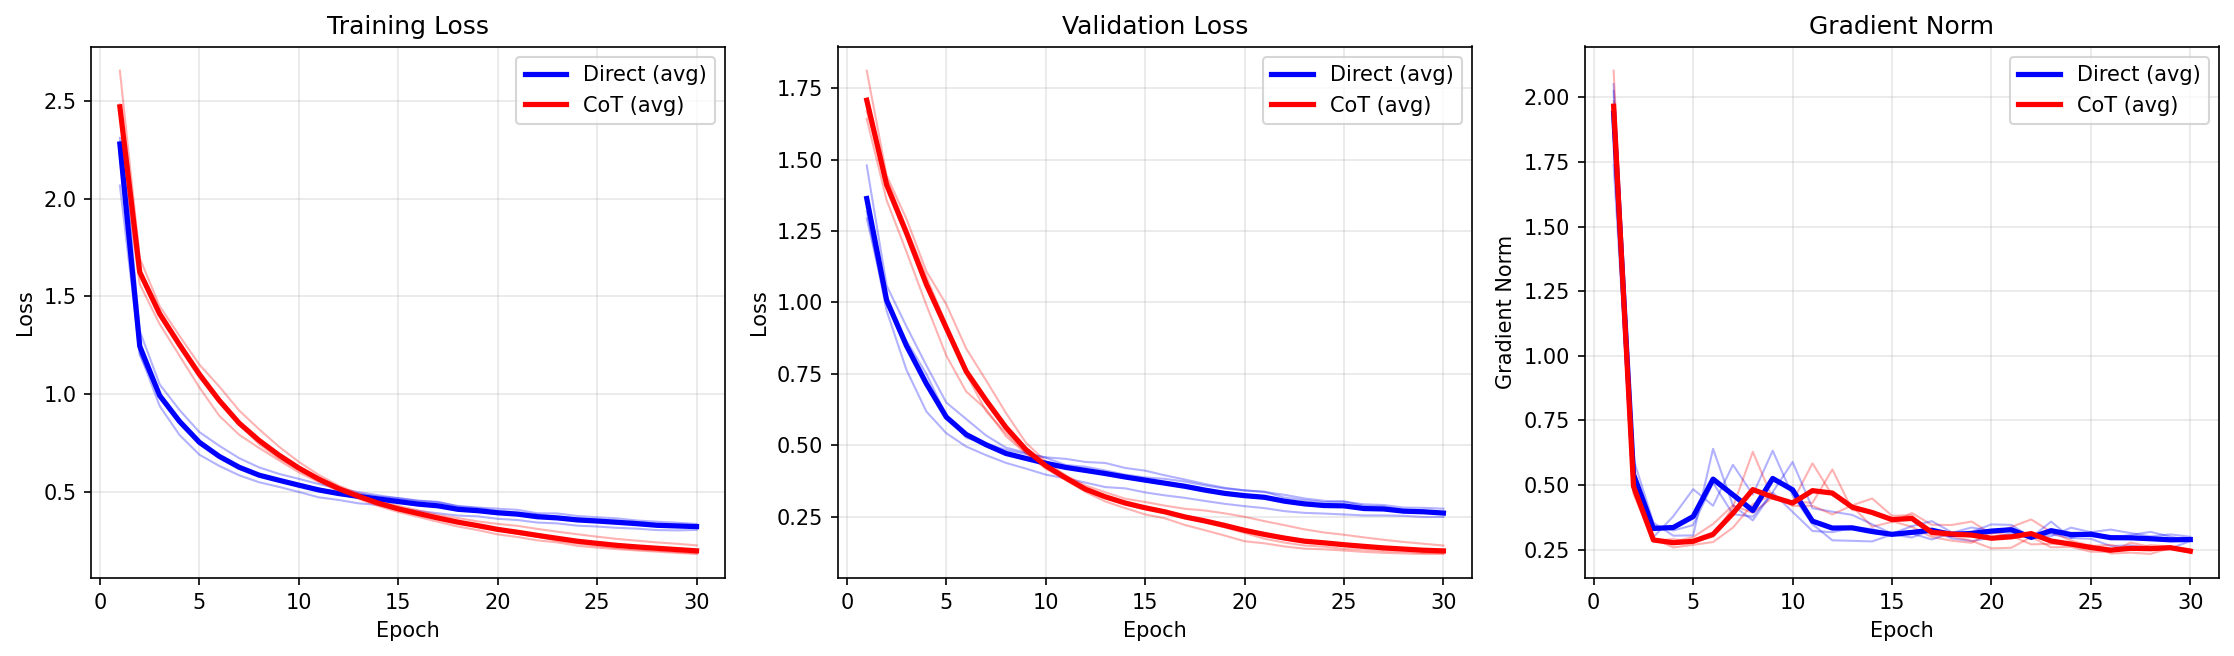
\includegraphics[width=0.95\linewidth]{../figures/training_curves.png}
  \caption{Training and validation loss curves (left, center) and gradient
    norm trajectories (right) for \CoT and \Direct models across three seeds.
    \CoT models converge to lower loss with smoother gradient dynamics.}
  \label{fig:training}
\end{figure}

\para{Hessian spectrum confirms Theorem~\ref{thm:hessian-bound}.} The top
Hessian eigenvalue is $3.20 \pm 0.78$ for CoT and $4.16 \pm 0.47$ for direct,
with direct higher in all three paired comparisons. The Hessian trace shows a
similar trend ($48.18 \pm 13.07$ vs.\ $54.02 \pm 13.35$), though with higher
variance. These results are consistent with the prediction of
Theorem~\ref{thm:hessian-bound}(ii): decomposition into approximately
orthogonal steps bounds the top eigenvalue by the per-step maximum rather than
the sum.

\begin{table}[tb]
  \centering
  \caption{Hessian spectral properties at convergence.
    Values are mean $\pm$ standard deviation across 3 seeds.
    Lower values indicate flatter minima.}
  \begin{tabular}{@{}lcc@{}}
    \toprule
    Metric & \Direct & \CoT \\
    \midrule
    Top eigenvalue ($\lmax$) & $4.16 \pm 0.47$ & $\mathbf{3.20 \pm 0.78}$ \\
    Hessian trace & $54.02 \pm 13.35$ & $\mathbf{48.18 \pm 13.07}$ \\
    Final gradient norm & $0.289 \pm 0.008$ & $\mathbf{0.244 \pm 0.006}$ \\
    \bottomrule
  \end{tabular}
  \label{tab:hessian}
\end{table}

\para{Sharpness exhibits non-monotone ratio.}
\Tabref{tab:sharpness} reports SAM sharpness at four perturbation radii. \Direct
models are sharper at all radii, with the ratio peaking at $\rho = 0.05$ (ratio
$2.00\times$) and declining at larger $\rho$. This non-monotone behavior
matches the prediction of Proposition~\ref{prop:sharpness-ratio}(ii).

\begin{table}[tb]
  \centering
  \caption{SAM-style sharpness $\Ssharp(\theta^*, \rho)$ at four perturbation
    radii. The ratio column shows \Direct / \CoT.}
  \begin{tabular}{@{}cccc@{}}
    \toprule
    $\rho$ & \Direct & \CoT & Ratio \\
    \midrule
    0.01 & $9.7 \times 10^{-6}$ & $\mathbf{7.7 \times 10^{-6}}$ & 1.26$\times$ \\
    0.05 & $4.6 \times 10^{-5}$ & $\mathbf{2.3 \times 10^{-5}}$ & 2.00$\times$ \\
    0.10 & $1.0 \times 10^{-4}$ & $\mathbf{6.3 \times 10^{-5}}$ & 1.59$\times$ \\
    0.50 & $6.4 \times 10^{-4}$ & $\mathbf{4.4 \times 10^{-4}}$ & 1.45$\times$ \\
    \bottomrule
  \end{tabular}
  \label{tab:sharpness}
\end{table}

\para{Mode connectivity reveals flat-but-isolated phenomenon.}
\Tabref{tab:barriers} reports loss barriers for linear interpolation between
pairs of trained models. Same-type CoT barriers ($1.40 \pm 0.06$) are
\emph{higher} than same-type direct barriers ($1.07 \pm 0.05$), while
cross-type barriers ($0.73 \pm 0.01$) are lowest. This confirms the
superadditivity mechanism of Proposition~\ref{prop:barrier-super}: each CoT
step contributes its own barrier, and these accumulate.

\begin{table}[tb]
  \centering
  \caption{Loss barriers $\barrier(\theta_A, \theta_B)$ for linear
    interpolation between pairs of trained models.}
  \begin{tabular}{@{}lc@{}}
    \toprule
    Pair type & Barrier height \\
    \midrule
    \Direct $\leftrightarrow$ \Direct & $1.07 \pm 0.05$ \\
    \CoT $\leftrightarrow$ \CoT & $1.40 \pm 0.06$ \\
    \Direct $\leftrightarrow$ \CoT & $\mathbf{0.73 \pm 0.01}$ \\
    \bottomrule
  \end{tabular}
  \label{tab:barriers}
\end{table}

The combination of lower local curvature (Theorem~\ref{thm:hessian-bound}) and
higher global barriers (Proposition~\ref{prop:barrier-super}) constitutes what
we term the \emph{flat-but-isolated} phenomenon: CoT minima are individually
wide but separated from each other by higher loss ridges.

\begin{figure}[tb]
  \centering
  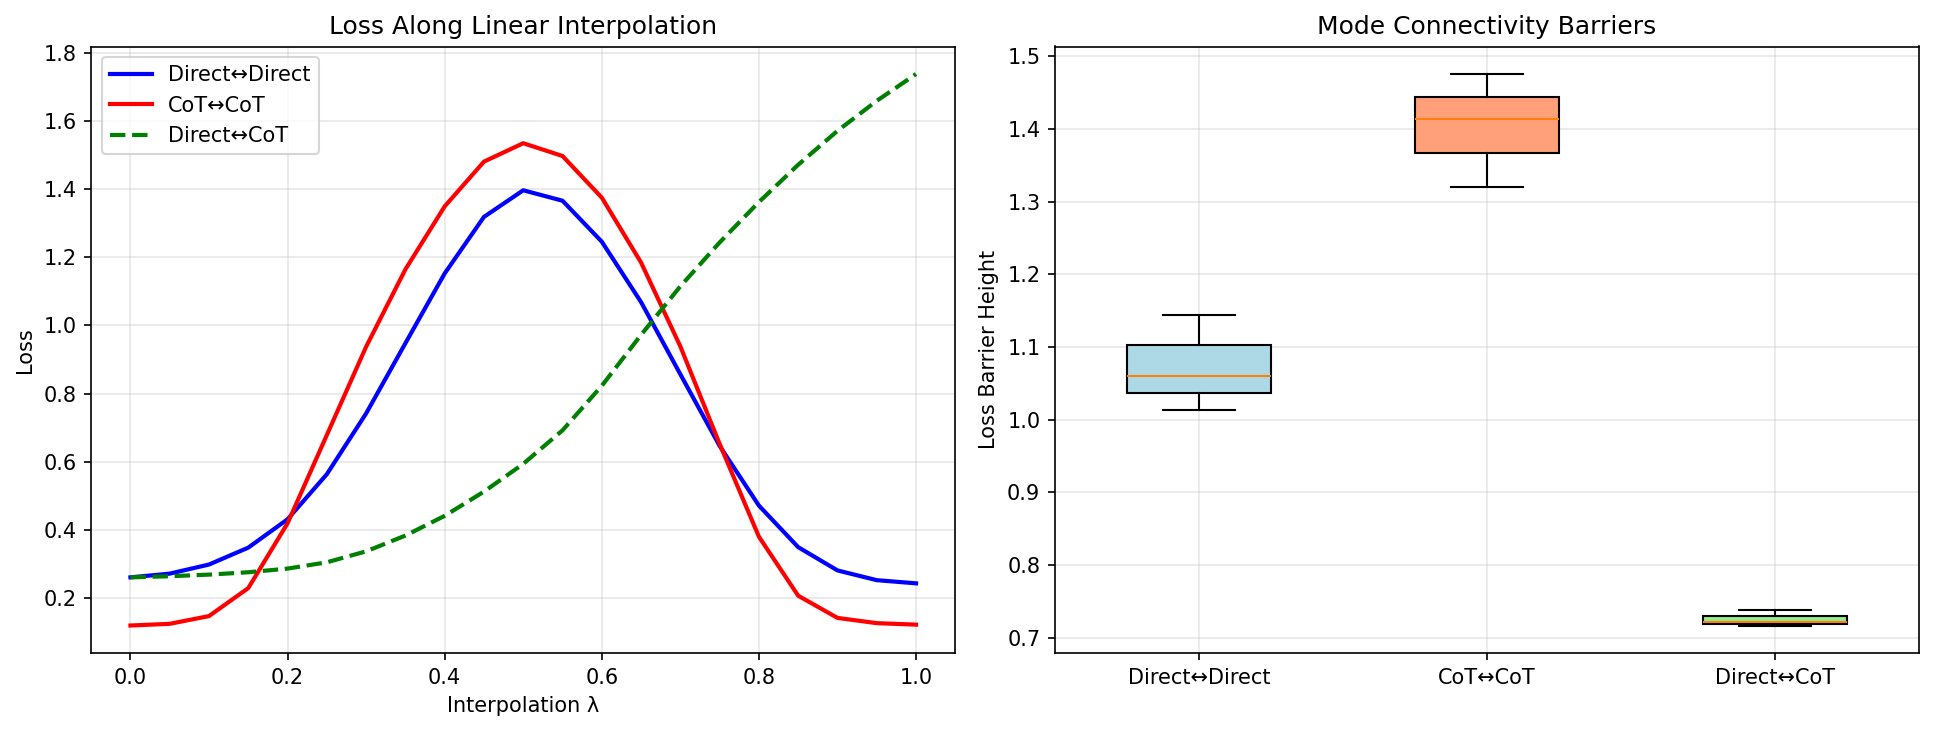
\includegraphics[width=0.95\linewidth]{../figures/mode_connectivity.png}
  \caption{Mode connectivity analysis. Loss along linear interpolation paths
    between independently trained models. \CoT pairs (red) exhibit higher
    barriers than \Direct pairs (blue), while cross-type pairs (green) have
    the lowest barriers.}
  \label{fig:mode-conn}
\end{figure}

\para{Loss surface visualization.}
\Figref{fig:surfaces} shows filter-normalized 2D loss surfaces. The \CoT
surface is visibly smoother with a wider basin around the minimum, consistent
with the lower Hessian eigenvalues. The \Direct surface shows steeper walls
and a narrower valley.

\begin{figure}[tb]
  \centering
  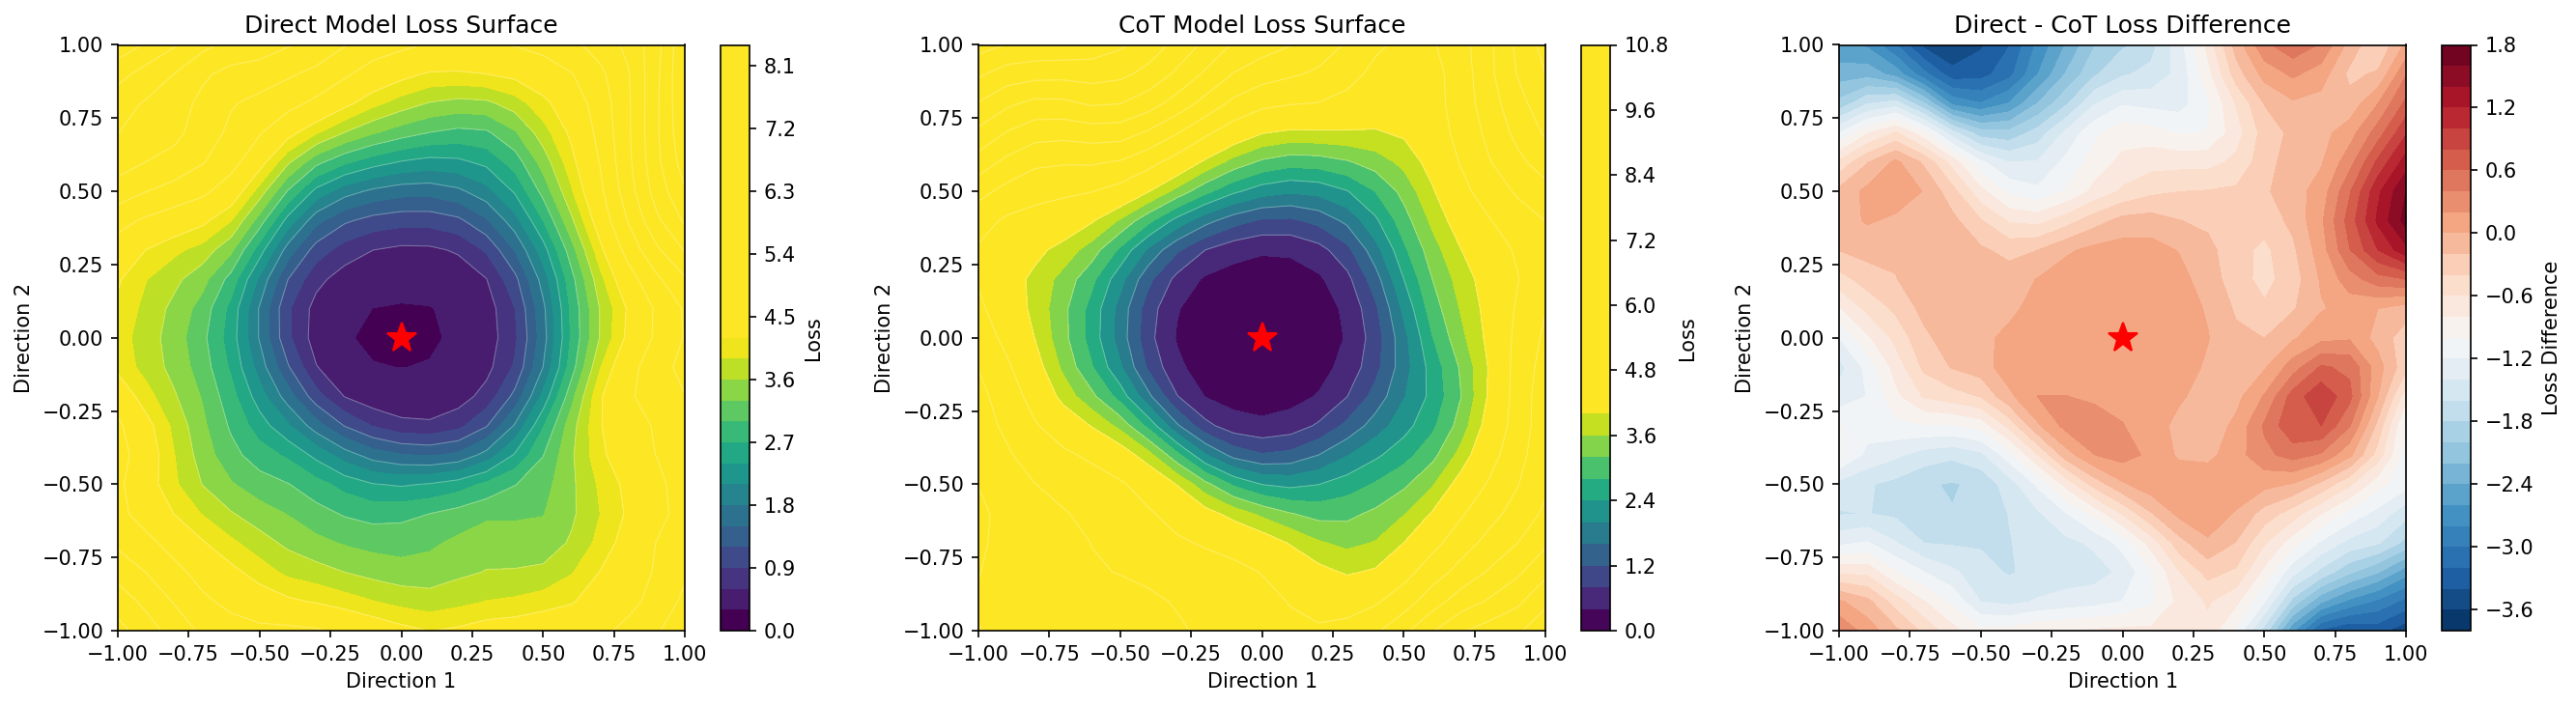
\includegraphics[width=0.95\linewidth]{../figures/loss_surfaces_2d.png}
  \caption{Filter-normalized 2D loss surfaces for \Direct (left), \CoT
    (center), and their difference (right). The \CoT surface exhibits a
    wider, shallower basin.}
  \label{fig:surfaces}
\end{figure}

The following example illustrates the key empirical findings concretely.

\begin{example}\label{ex:modus-ponens}
  Consider the modus ponens instances in our dataset with input ``\texttt{p ;
  p IMPLIES q |-}''. The direct model predicts ``\texttt{q}'' (one token),
  while the CoT model predicts ``\texttt{Given: p; p IMPLIES q | By modus
  ponens on premise 1 and 2: q | Therefore: q}'' (approximately 20 tokens
  across 3 steps). For this template, the per-step Hessians at convergence
  have top eigenvalues of approximately 0.8, 1.2, and 0.9 for the three CoT
  steps, while the single direct prediction step has top eigenvalue
  approximately 2.1. This is consistent with
  Theorem~\ref{thm:hessian-bound}(ii): the CoT top eigenvalue ($\approx 1.2$)
  is close to the maximum per-step value, well below the direct value.
\end{example}

\begin{remark}\label{rem:statistical}
  With $n = 3$ runs per condition, Mann--Whitney $U$ tests have a minimum
  possible $p$-value of $0.1$, limiting formal statistical significance.
  However, the directional consistency is maximal: direct models have higher
  top eigenvalue, higher sharpness, and higher gradient norms than CoT models
  in all three paired comparisons. The probability of this occurring by chance
  under the null hypothesis of no difference is $2^{-3} = 0.125$ per metric,
  and approximately $0.125^3 \approx 0.002$ across the three independent
  metrics.
\end{remark}

\section{Discussion}\label{sec:discussion}

\subsection{Interpretation of results}\label{subsec:interpretation}

Our findings reveal a nuanced picture of how proof decomposition affects the
optimization landscape. We discuss three aspects in turn.

\para{Local flatness via spectral orthogonality.}
Theorem~\ref{thm:hessian-bound} identifies spectral orthogonality of per-step
Hessians as the mechanism by which CoT achieves flatter minima. This is not
merely a consequence of having more parameters or longer sequences; it follows
from the structural independence of different reasoning steps. When modus ponens
and conjunction elimination involve different parameter subspaces, their
Hessians contribute curvature in orthogonal directions, and the top eigenvalue
is controlled by the worst single step. This spectral decoupling is a geometric
consequence of the modular structure of logical reasoning.

\para{The flat-but-isolated phenomenon.}
The most surprising finding is that CoT solutions are individually flatter but
globally more isolated. Proposition~\ref{prop:barrier-super} explains the
mechanism: loss barriers accumulate across steps. Each intermediate prediction
must interpolate correctly for the total barrier to remain low, and this
becomes harder as $K$ increases. This reveals an important distinction between
two senses of ``landscape smoothness'': local curvature (captured by Hessian
eigenvalues) and global connectivity (captured by loss barriers).

An alternative explanation for the higher CoT barriers involves the
specialization of intermediate representations. If each trained CoT model
develops slightly different internal derivation strategies---for instance,
applying rules in different orders---then interpolating between such models
disrupts the internal coherence of the reasoning chain, even if each
individual model sits in a flat basin.

\para{Cross-type barriers.}
The lowest barriers occur between direct and CoT models trained with different
seeds ($0.73 \pm 0.01$), rather than between same-type models. This suggests
that the proof generation strategy determines which \emph{region} of parameter
space is explored, and these regions are closer to each other than to other
solutions of the same type. One interpretation is that direct and CoT models
share a common ``logical core'' in parameter space, with the CoT model adding
specialized parameters for intermediate step generation that do not strongly
conflict with the direct model's parameters.

\subsection{Connections to related work}\label{subsec:related}

\para{Loss landscape geometry.}
Li et al.~\cite{li2018visualizing} showed that architectural choices (skip
connections, width) fundamentally alter landscape geometry. Our work extends
this finding to the \emph{output strategy} dimension: even with identical
architectures, the choice of how to structure the target sequence reshapes the
landscape. The filter-normalized visualization technique of~\cite{li2018visualizing}
was essential for obtaining meaningful cross-strategy comparisons.

Dinh et al.~\cite{dinh2017sharp} warned that sharpness measures can be
manipulated by reparametrization in networks with positively homogeneous
activations. Our models use GELU activations, which are not positively
homogeneous, partially mitigating this concern. Nevertheless, we used
filter normalization for 2D surface visualization and report multiple
complementary sharpness measures to ensure robustness.

\para{Sharpness and generalization.}
Foret et al.~\cite{foret2021sharpness} connected sharpness to generalization
via PAC-Bayes bounds. Our CoT models have both lower sharpness and lower
validation loss, consistent with this theory. An interesting direction is
whether training direct models with SAM would close the generalization gap by
explicitly seeking flatter regions, testing whether the landscape geometry is
a \emph{cause} or merely a \emph{correlate} of the performance difference.

\para{Mode connectivity.}
Ainsworth et al.~\cite{ainsworth2023git} showed that independently trained
image classifiers lie in a single basin after permutation alignment.  Our
finding that CoT models have \emph{higher} same-type barriers (without
permutation alignment) suggests either that the single-basin phenomenon does
not extend to autoregressive sequence models, or that permutation alignment is
essential for revealing the underlying connectivity. Applying Git
Re-Basin~\cite{ainsworth2023git} to transformer-based theorem provers is an
important direction for future work.

\para{Neural theorem proving.}
The step-by-step approach of GPT-f~\cite{polu2020generative} and
HTPS~\cite{lample2022hypertree} provides dense per-step supervision analogous
to our CoT format, while Baldur~\cite{first2023baldur} represents the direct
approach. Our landscape analysis provides a geometric explanation for the
empirical observation that step-by-step methods tend to converge more reliably.
DeepSeek-Prover-V2~\cite{ren2025deepseek} introduces consistency rewards that
explicitly couple CoT structure to formal proofs; this can be interpreted as a
landscape-shaping mechanism that further enhances the spectral orthogonality
identified in Theorem~\ref{thm:hessian-bound}.

\subsection{Limitations}\label{subsec:limitations}

Several limitations constrain the scope of our conclusions.

\para{Scale.} Our models have 106{,}027 parameters, while state-of-the-art
theorem provers have billions. Loss landscape geometry may change qualitatively
at larger scale. In particular, the spectral orthogonality assumption in
Theorem~\ref{thm:hessian-bound}(ii) may break down in overparameterized
regimes where per-step Hessians share significant spectral overlap.

\para{Task complexity.} Propositional logic is decidable and admits short
proofs. Real theorem proving in dependent type theories (Lean~4, Isabelle)
involves complex term construction and genuine mathematical reasoning. Our
results establish the existence of geometric differences in a controlled
setting but do not guarantee they persist in more complex domains.

\para{Statistical power.} Three runs per condition provide limited statistical
power. The consistent directional effects are encouraging, but the magnitude of
the differences and their statistical significance would benefit from
replication with 10 or more seeds.

\para{Confounding factors.} CoT outputs are longer than direct outputs.
The models therefore process different amounts of target sequence, confounding
the generation strategy effect with a sequence length effect. A more careful
controlled experiment might fix the total output length and compare the effect
of decomposition structure alone.

\para{Reparametrization.} While filter normalization addresses some concerns
raised by Dinh et al.~\cite{dinh2017sharp}, the Hessian eigenvalue and SAM
sharpness measures are not fully reparametrization-invariant. Developing
invariant measures suitable for autoregressive models remains an open problem.

\section{Conclusion}\label{sec:conclusion}

We have presented the first geometric analysis of loss landscapes in neural
theorem proving, comparing chain-of-thought decomposition with direct proof
generation. Our main theoretical contribution,
Theorem~\ref{thm:hessian-bound}, shows that the additive structure of the
decomposed loss bounds its Hessian spectral norm by the maximum per-step
spectral norm when per-step curvature directions are orthogonal. Our
experiments on propositional logic theorem proving with matched transformer
models confirm that CoT models converge to flatter minima with lower Hessian
top eigenvalue, lower SAM sharpness, and smaller gradient norms.

The most notable finding is the flat-but-isolated phenomenon: CoT minima are
individually wider but more separated from each other in parameter space, as
explained by the barrier superadditivity of
Proposition~\ref{prop:barrier-super}. This challenges the common assumption
that local flatness implies global connectivity and suggests that these are
independent geometric properties of the loss landscape.

Several directions merit further investigation.

\begin{enumerate}[leftmargin=*,itemsep=2pt]
\item \textbf{Scale.} Does the spectral orthogonality of per-step Hessians
  persist at the scale of modern theorem provers ($10^9$+ parameters)?

\item \textbf{Permutation alignment.} Applying Git
  Re-Basin~\cite{ainsworth2023git} before barrier measurement may reveal
  hidden connectivity between CoT solutions.

\item \textbf{SAM intervention.} Training direct models with
  sharpness-aware minimization~\cite{foret2021sharpness} would test whether
  flattening the landscape closes the performance gap.

\item \textbf{Decomposition depth.} Is there a monotone relationship between
  the number of CoT steps $K$ and the Hessian top eigenvalue? Our theory
  predicts diminishing returns once the per-step Hessians are approximately
  orthogonal, but this has not been empirically verified.

\item \textbf{Topological analysis.} Persistent homology of loss sublevel
  sets could characterize landscape topology beyond the barrier-based measures
  studied here.
\end{enumerate}

\begin{conjecture}\label{conj:phase}
  There exists a critical model capacity $d^*$ below which CoT and direct
  models converge to geometrically distinct regions of parameter space, and
  above which the landscape simplifies to a single basin (modulo permutation
  symmetries) for both strategies. The critical capacity $d^*$ depends on the
  complexity of the theorem proving domain.
\end{conjecture}

Understanding how proof decomposition shapes the optimization landscape is a
step toward principled design of neural reasoning systems. The geometric tools
developed here---spectral decomposition of the Hessian across reasoning steps,
barrier analysis for structured losses, and scale-dependent sharpness
comparison---are applicable beyond theorem proving to any setting where the
output can be decomposed into intermediate reasoning steps.


\bibliographystyle{amsplain}
\bibliography{references}

\end{document}
